\section{Using the spreadsheet application}
\label{sec:using}

The spreadsheet application can be run by running Scala on the class
\texttt{spreadsheet.SpreadsheetApp}, providing the name of the script to use.
The application uses the Scala Swing library, so the jar file must be on the
classpath.  I use the following command (except all on one line): {\small
\begin{verbatim}
scala -cp .:scala-swing_2.13-3.0.0.jar 
  spreadsheet.SpreadsheetApp factorials.dir 
\end{verbatim}
}
Optionally, the name of a CSV file can also be provided, giving values to load
into the spreadsheet. 

Values can be entered into the spreadsheet in the normal way.  The script is
run automatically each time the user enters a value.
Figure~\ref{fig:screenshot} gives a screenshot of the window after the user
has input values into the first three cells in column~|A|.  Cells with a
purple background are user inputs; cells with a green background contain values
written by the script, with the currently selected cell in a darker shade.

\framebox{Update screenshots}

\begin{figure}[thp]
\centering
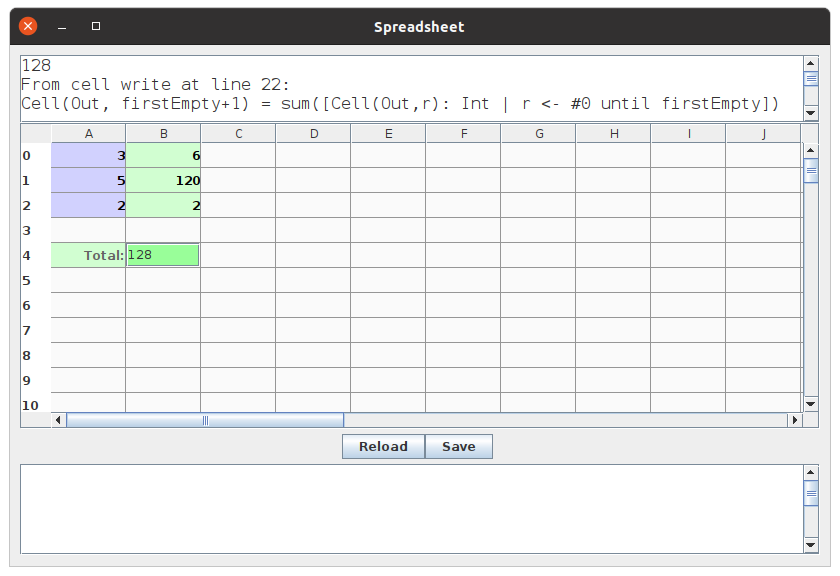
\includegraphics[scale=0.46]{screenshot.png}
\caption{The spreadsheet application window.}
\label{fig:screenshot}
\end{figure}

The top panel in the window, known as the \emph{selection panel}. gives
information about the selected cell.  Here it shows that the cell contains the
value~128, that the value came from a cell write at line~\ref{line:write-sum};
it also gives the corresponding code.

%%%%%

As with any programming language, errors can occur, which can be detected
either when the script is type checked, or when the script is executed.

As an example of a type error, suppose we change line~\ref{line:factorial} of
the script to the following:
%
\begin{scala}
def fact(n: Int): Int = if(n <= 1.0) 1 else n*fact(n-1)
\end{scala}
%
This is a type error, because it compares the |Int|~|n| with the floating
point number~|1.0|.  Figure~\ref{fig:screenshot-type-error} shows what happens
when the script is re-loaded (via the ``Reload'' button).  The bottom panel,
known as the \emph{error panel}, gives information about each error.  Here it
indicates that the script expected an |Int| but found a |Float| at
line~\ref{line:factorial}, and that the erroneous term was~|1.0|; it also gives
enclosing code at various levels.

\begin{figure}[thp]
\centering
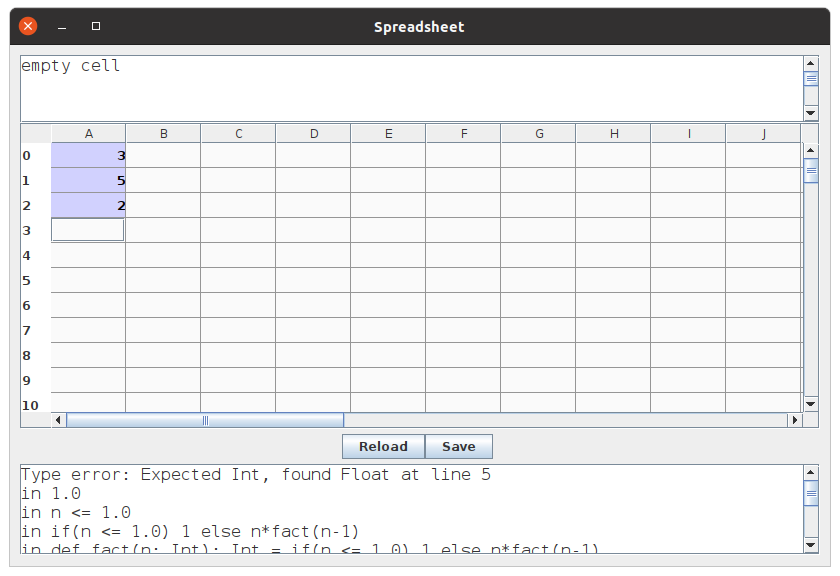
\includegraphics[scale=0.46]{screenshot-type-error.png}
\caption{The spreadsheet application indicating a type error.}
\label{fig:screenshot-type-error}
\end{figure}

%%%%%

Execution-time errors include errors common in other programming languages,
such as division by zero, or taking the head of an empty list.

A non-standard form of error occurs when the script reads a value from a cell
that is not of the expected type.  For example, suppose we enter the string
|three| into cell |#A0|; then the error panel displays the following error:
%
\begin{trivlist}
\item[]
\footnotesize
\begin{verbatim}
Cannot match String in cell #A0 at line 12
in "Cell(c,r) match{ case Empty => r; case _: Int => firstEmptyInCol(c, r+1) }"
in "firstEmptyInCol(In, #0)"
in "val firstEmpty = firstEmptyInCol(In, #0)"
\end{verbatim}
\end{trivlist}
%
This shows that the pattern matching at line 12 fails when given a string. 

Similar errors can occur outside pattern matching.  Suppose we change the
definition of |firstEmptyInCol| as follows.
%
\begin{scala}
def firstEmptyInCol(c: Column, r: Row): Row =
  Cell(c,r) match{ case Empty => r; case _ => firstEmptyInCol(c, r+1) }
\end{scala}
%
The pattern ``|_|'' matches any value, so the pattern matching will succeed.
However, now other errors occur, as illustrated in
Figure~\ref{fig:screenshot-read-error}, where cells with a pink background
represent errors.  The error panel indicates that the cell~|#A0| read at
line~18 found a |String| when an |Int| was expected.  The same information is
included in the selection panel, since cell |#B0| is selected.  The bottom of
the error panel also explains an error corresponding to the write
of cell~|#B4| (this requires scrolling to read fully).

\begin{figure}[thp]
\centering
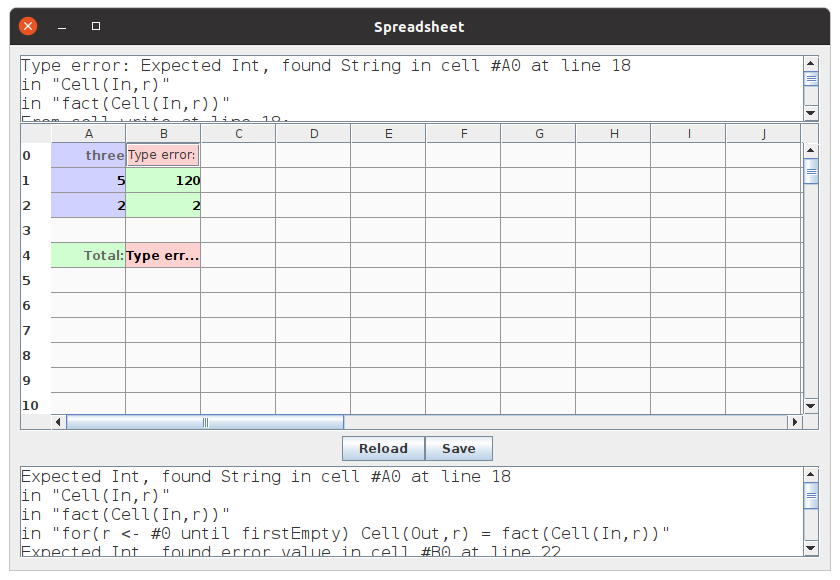
\includegraphics[scale=0.46]{screenshot-read-error.png}
\caption{The spreadsheet application indicating a cell read error.}
\label{fig:screenshot-read-error}
\end{figure}

%%%%%  IMPROVE************* Give example of assertion error. 

The application partitions cells into \emph{input cells}, where the user has
provided input, \emph{output cells}, written to by the script, and \emph{empty
  cells}.  Any attempt to write to an input cell is considered an error and
blocked: this prevents an erroneous script from overwriting user data.
Likewise, an attempt to write to an output cell for a second time is
considered an error. 

The ``Save'' button on the spreadsheet can be used to store the contents of
input cells in a CSV file.  
